\section{Emulation of the CMS search}\label{sec:emulation}

The emulated event selection is summarized as follows,
\begin{itemize}
\item Events with two isolated photons with $\pt>25$\GeV and
  $|\eta|<1.44$ are selected. As in Ref.~\cite{CMSPhoton}, the photon
  isolation variables, $I_{\gamma}$, $I_{\mathrm{n}}$, and $I_{\pi}$, are
  computed by summing the transverse momenta of photons, neutral
  hadrons, and charged hadrons, respectively, inside an isolation
  cone of radius $\Delta R=0.3$ around the selected photon. The photon
  isolation requirements on these variables
  are shown in Tab~\ref{tab:isolation}. An additional photon selection
  efficiency is applied in \textsc{Delphes} such that isolated photons with $\pt<10$\GeV ($\pt\geq10$\GeV) are
  randomly selected with 94\% (98\%) efficiency.
\begin{table}\centering
\caption{\label{tab:isolation}Photon isolation requirements, as in
  Ref~\cite{CMSPhoton}. The photon isolation variables, $I_{\gamma}$, $I_{\mathrm{n}}$, and $I_{\pi}$, are
  computed by summing the transverse momenta of photons, neutral
  hadrons, and charged hadrons, respectively, inside an isolation
  cone of radius $\Delta R=0.3$ around the selected photon.}
%\begin{ruledtabular}
\begin{tabular}{lc|r}\hline\hline
 \multirow{2}{*}{$I_{\gamma}$} & barrel & $1.3\GeV + 0.005\pt^{\gamma}$\\
 & endcap & -- \\\hline
 \multirow{2}{*}{$I_{\mathrm{n}}$} & barrel & $3.5\GeV+ 0.04\pt^{\gamma}$\\
 & endcap &  $2.9\GeV+ 0.04\pt^{\gamma}$ \\\hline
 \multirow{2}{*}{$I_{\pi}$} & barrel & $2.6\GeV$\\
 & endcap &  $2.3\GeV$ \\\hline\hline
\end{tabular}
%\end{ruledtabular}
\end{table}
\item Events with one $\PH$ candidate with $\pt>20$ GeV are selected. A pair of selected
  photons is considered an $\PH$ candidate if at
  least one photon has $\pt>40$\GeV and the diphoton mass
  $m_{\Pgg\Pgg}>100$\GeV. If the event contains more than one $\PH$ candidate,
  the one with the highest scalar sum $\pt$ of the two photons is selected. 
\item Jets are reconstructed using the \FASTJET~\cite{fastjet} implementation
  of the anti-$\kt$~\cite{antikt} algorithm with jet radius parameter $R=0.5$.
\item Events with at least one jet with $\pt>30$ GeV and $|\eta|<3.0$
  are selected.
\item An emulation of the ``medium'' requirement (mistag probability of
  1\% and \cPqb-tag efficiency of $\sim 68\%$) of the combined secondary vertex (CSV) \cPqb-tagging
  algorithm is used to identify \cPqb-jets~\cite{btag8TeV}.
\item A $\bbbar$ candidate pair is identified if both jets satisfy the medium requirement of
  the \cPqb-tagging algorithm (note: the CMS analysis requires only one to
  satisfy the medium requirement, while both are required to satisfy
  the loose requirement).
\item The $\bbbar$ candidate pair with the mass closest to 125\GeV or 91.2\GeV is chosen as the $\PH\to
  \bbbar$ or $\PZ\to \bbbar$ candidate, respectively.
\item The razor variable \MR, calculated from two megajets~\cite{razorPRD} is required to be greater than
  $150\GeV$. All possible combinations of the reconstructed jets and
the $\PH(\Pgg\Pgg)$ candidate are clustered to form megajets. The pair of megajets that
minimizes the sum in quadrature of the invariant masses of the two megajets is selected.
\end{itemize}

After this baseline selection, events are categorized according to the
following requirements,
\begin{itemize}
\item \texttt{HighPt}: all events with an $\PH\to\Pgg\Pgg$ candidate
  with $p_{T}>110$\GeV. 
\item \texttt{Hbb}: remaining events with a $\PH\to \bbbar$ candidate
  with mass $110\geq m_{\bbbar}\geq 140$\GeV. 
\item \texttt{Zbb}: remaining events with a $\PZ\to \bbbar$ candidate
  with mass $76\geq m_{\bbbar}\geq 106$\GeV. 
\item \texttt{HighRes}: 70\% of remaining events after the
  \texttt{Zbb} selection (emulating the efficiency of the ``high-resolution photon'' selection).
\item \texttt{LowRes}: all remaining events. 
\end{itemize}
We assume the breakdown of events between the \texttt{HighRes} box and \texttt{LowRes}
box is 70\%-to-30\% after the \texttt{Zbb} selection. This
is based on the following observations:  (i) CMS categorizes events in the \texttt{HighRes} box if
both photons in the event satisfy $\sigma_E/E < 0.015$, where $\sigma_E/E$ is the estimated
relative energy resolution, and categorizes events in the
\texttt{LowRes} box otherwise, (ii) CMS observes a similar
70\%-to-30\% breakdown for both SM Higgs production and
electroweak SUSY processes in Monte Carlo
simulation~\cite{RazorHgaga}, and (iii) we expect this breakdown to be
model-independent assuming both photons are real and come from the
decay of a Higgs boson, as it is based on the properties of such photons
detected in CMS and not on the details of the model.

%Given the difficulty of emulating the high-resolution requirement
%(both photons must satisfy $\sigma_E/E<0.015$, where $\sigma_E/E$ is the relative
%energy resolution for the identified photons) for the \texttt{HighRes}
%box, and the high efficiency of this requirement for \emph{real}
%photons, we make the assumption that all of our benchmark signal events (which contain
%a real $\PH\to\Pgg\Pgg$) pass this requirement and thus no signal events
%fall into the \texttt{LowRes} box.

Finally, the search region selection is as follows,
\begin{itemize}
\item The search region in the $m_{\Pgg\Pgg}$ distribution is
    defined by $(125 - 2\sigma_{\mathrm{eff}},
    126+2\sigma_{\mathrm{eff}})$ in each event category, where
    $\sigma_{\mathrm{eff}}$ is defined such that $\sim68\%$ of Higgs
    boson events fall in an interval of $\pm\sigma_{\mathrm{eff}}$
    around the nominal $m_\PH$ value. Following this procedure using
    our generated and simulated signal samples, we derive
    $\sigma_{\mathrm{eff}}$ to be 3.8\GeV in the \texttt{HighPt} box
    and 2.2\GeV in the \texttt{HighRes} and \texttt{LowRes}
    boxes. For the \texttt{Hbb} and \texttt{Zbb} boxes, due to the low
    number of selected signal events, we use the overall average value
    of 2.8\GeV. 
    %$\sigma_{\mathrm{eff}}=1.46$\GeV in the \texttt{HighRes} box, 
   %$\sigma_{\mathrm{eff}}=1.56$\GeV in the \texttt{HighPt} box, and $\sigma_{\mathrm{eff}}=2$\GeV in the
%\texttt{Hbb} and \texttt{Zbb} boxes.
\end{itemize}
We note that these $\sigma_{\mathrm{eff}}$ values are larger than the
    corresponding ones in Ref.~\cite{RazorHgaga}. This is due to the
    larger width observed for the diphoton mass distribution in Higgs
    boson events simulated and reconstructed with \textsc{Delphes},
    compared to official CMS software. This implies the effective
    diphoton mass resolution when using \textsc{Delphes} is larger than in the
    real CMS detector. We attempt to account for this with a
    modification explained in Sec.~\ref{sec:validation}.

\section{Bayesian Statistical Interpretation}\label{sec:bayes}

We model the likelihood according to a Poisson density,
considering the expected background yield (with associated
uncertainty), the expected signal yield (for a given signal cross
section), and the observed yield. The background uncertainty is modeled with a gamma density. The
background yields and the corresponding uncertainties are taken from the tables provided
in Ref.~\cite{RazorHgaga}. To take into account systematic
uncertainties on the signal, we assign a 30\% uncertainty (assuming a
log-normal density) on the signal strength, a multiplicative
factor modifying the signal cross section. We then derive the
posterior density for the signal cross section $\sigma$ as:
\begin{equation}
p(\sigma|\mathrm{data}) \propto \mathcal L(\mathrm{data} |\sigma)p_0(\sigma)~,
\label{eqn:posterior}
\end{equation}
where $\mathcal L(\mathrm{data} |\sigma)$ is the likelihood and $p_0(\sigma)$ is the prior density taken to be
uniform. The likelihood is then
\begin{align}
\mathcal L(\mathrm{data} |\sigma)
  &=\int_{0}^{\infty}\mathrm{d}\mu~\mathrm{Ln}(\mu|\bar\mu,\delta\mu)\\
&\times\prod_{i=0}^{n_{\mathrm{bins}}}\int_0^{\infty} \mathrm{d}b_i
   \mathrm{Poisson}(n_i|L\mu\sigma\epsilon_i+ b_i)\nonumber\\
&\times\Gamma(b_i|\bar{b}_i,\delta b_i)~,
\label{eqn:likelihood}
\end{align}
where the product runs over the number of bins $n_{\mathrm{bins}}$; $n_i$ is the
observed yield in the $i^{\mathrm{th}}$ bin, $L$ is the integrated
luminosity, $b_i$ is the assumed value of the background yield in the
$i^{\mathrm{th}}$ bin and $\bar{b}_i\pm \delta b_i$ is its expected value
and the associated uncertainty; $\epsilon_i$ is the nominal value
of the signal efficiency times acceptance in the $i^{\mathrm{th}}$ bin; $\mu$ is the
signal strength, a nuisance parameter modifying the signal cross section
(nominally equal to $\bar\mu=1$ with a $\delta\mu=30\%$ uncertainty);
$\mathrm{Ln}(x|m,\delta)$ is the log-normal
distribution for $x$, parameterized such that $\mathrm{log}(m)$ is the
mean and $\mathrm{log}(1+m\delta)$ is the standard deviation of the
log of the distribution; $\Gamma(x|m,\delta)$ is the gamma
distribution for $x$, parameterized such that $m$ is the
mode and $\delta^2$ is the variance of the distribution. The 95\%
credibility level (CL) upper limit on the
signal cross section $\sigma_{\mathrm{up}}$ is obtained from the
posterior, such that 
\begin{equation}
\frac{\int_0^{\sigma_{\mathrm{up}}}\mathrm{d}\sigma~ p(\sigma|\mathrm{data})}{\int_0^{\infty}\mathrm{d}\sigma~ p(\sigma|\mathrm{data})} = 0.95~.
\end{equation}

We also utilize a signal significance measure defined by
\begin{align}
Z(\sigma) &= \mathrm{sign}[\log B_{10}(\mathrm{data},\sigma)]\sqrt{2|\log B_{10}(\mathrm{data},\sigma)|}~,
\label{eqn:zSig}
\end{align}
where 
\begin{align}
B_{10}(\mathrm{data},\sigma) &= \frac{\mathcal L(\mathrm{data}
  |\sigma,H_1)}{\mathcal L(\mathrm{data}
  |H_0)}
\label{eqn:localBayes}
\end{align}
is the \emph{local} Bayes factor for the data for a given signal cross
section $\sigma$, and $\mathcal L(\mathrm{data}
  |\sigma,H_1)$ and $\mathcal L(\mathrm{data}
  |H_0)$ are the likelihoods for the signal-plus-background ($H_1$) and
  background-only ($H_0$) hypotheses, respectively. As described in
  Ref.~\cite{CMS-PAS-SUS-15-010}, this
  measured is a signed Bayesian analog of the frequentist ``n-sigma.''
  For each signal model with specified masses, we scan the signal
  cross section $\sigma$ to find the maximum significance,
  which occurs at the mode of the posterior.

\section{Correction and Validation}\label{sec:validation}

%As explained Sec.~\ref{sec:emulation}, we find differences in the
As explained above, we find differences in the
performance of the emulated CMS detector and the real CMS detector,
e.g. the larger diphoton mass resolution. To take into account this
and other differences in the detector simulation and reconstruction performed by
\textsc{Delphes} and official CMS software, we conservatively double the
background uncertainties in each bin reported by CMS in Ref.~\cite{RazorHgaga} when evaluating the likelihood in
Eqn.~\ref{eqn:likelihood}. We find this conservative approach better
reproduces the observed and expected limits on a benchmark simplified
model.

To validate our emulation result, we produced 95\% CL
limits on the production cross section of an electroweak simplified
model of $\chipm_1\chiz_2$ production, followed by
the decays $\chipm_1\to \PW^{\pm}\chiz_1$,
$\chiz_2\to \PH\chiz_1$. For this model, CMS provided the 95\%
confidence level upper limits on the cross section assuming an LSP mass of
$m_{\chiz_1}=1\GeV$ and equal chargino and second neutralino
masses, $m_{\chipm_1}=m_{\chiz_2}$. 
%The posterior density
%for the production cross sections (assuming
%$m_{\tilde{\chi}_1^{\pm}}=200$\GeV) derived from our emulation of the CMS search are shown in
%figure~\ref{fig:TChiwhPosterior200}. 
The comparison between our result and the CMS result for this model is shown in
figure~\ref{fig:TChiwh1dLimit} as a function of $m_{\chipm_1}$.

%The expected upper limit from the emulation is consistently larger
%than the expected upper limit from the CMS result by a
%factor of $1.2$, $1.3$, and $1.5$ for $m_{\tilde{\chi}_1^{\pm}}
%=130$\GeV, $160$\GeV, and $200$\GeV, respectively. Similarly, the
%corresponding ratio of the observed upper limits are $1.4$, $1.7$, and
%$2.3$ for $m_{\tilde{\chi}_1^{\pm}}=130$\GeV, $160$\GeV, and $200$\GeV, respectively.

%\begin{figure}[htb]
%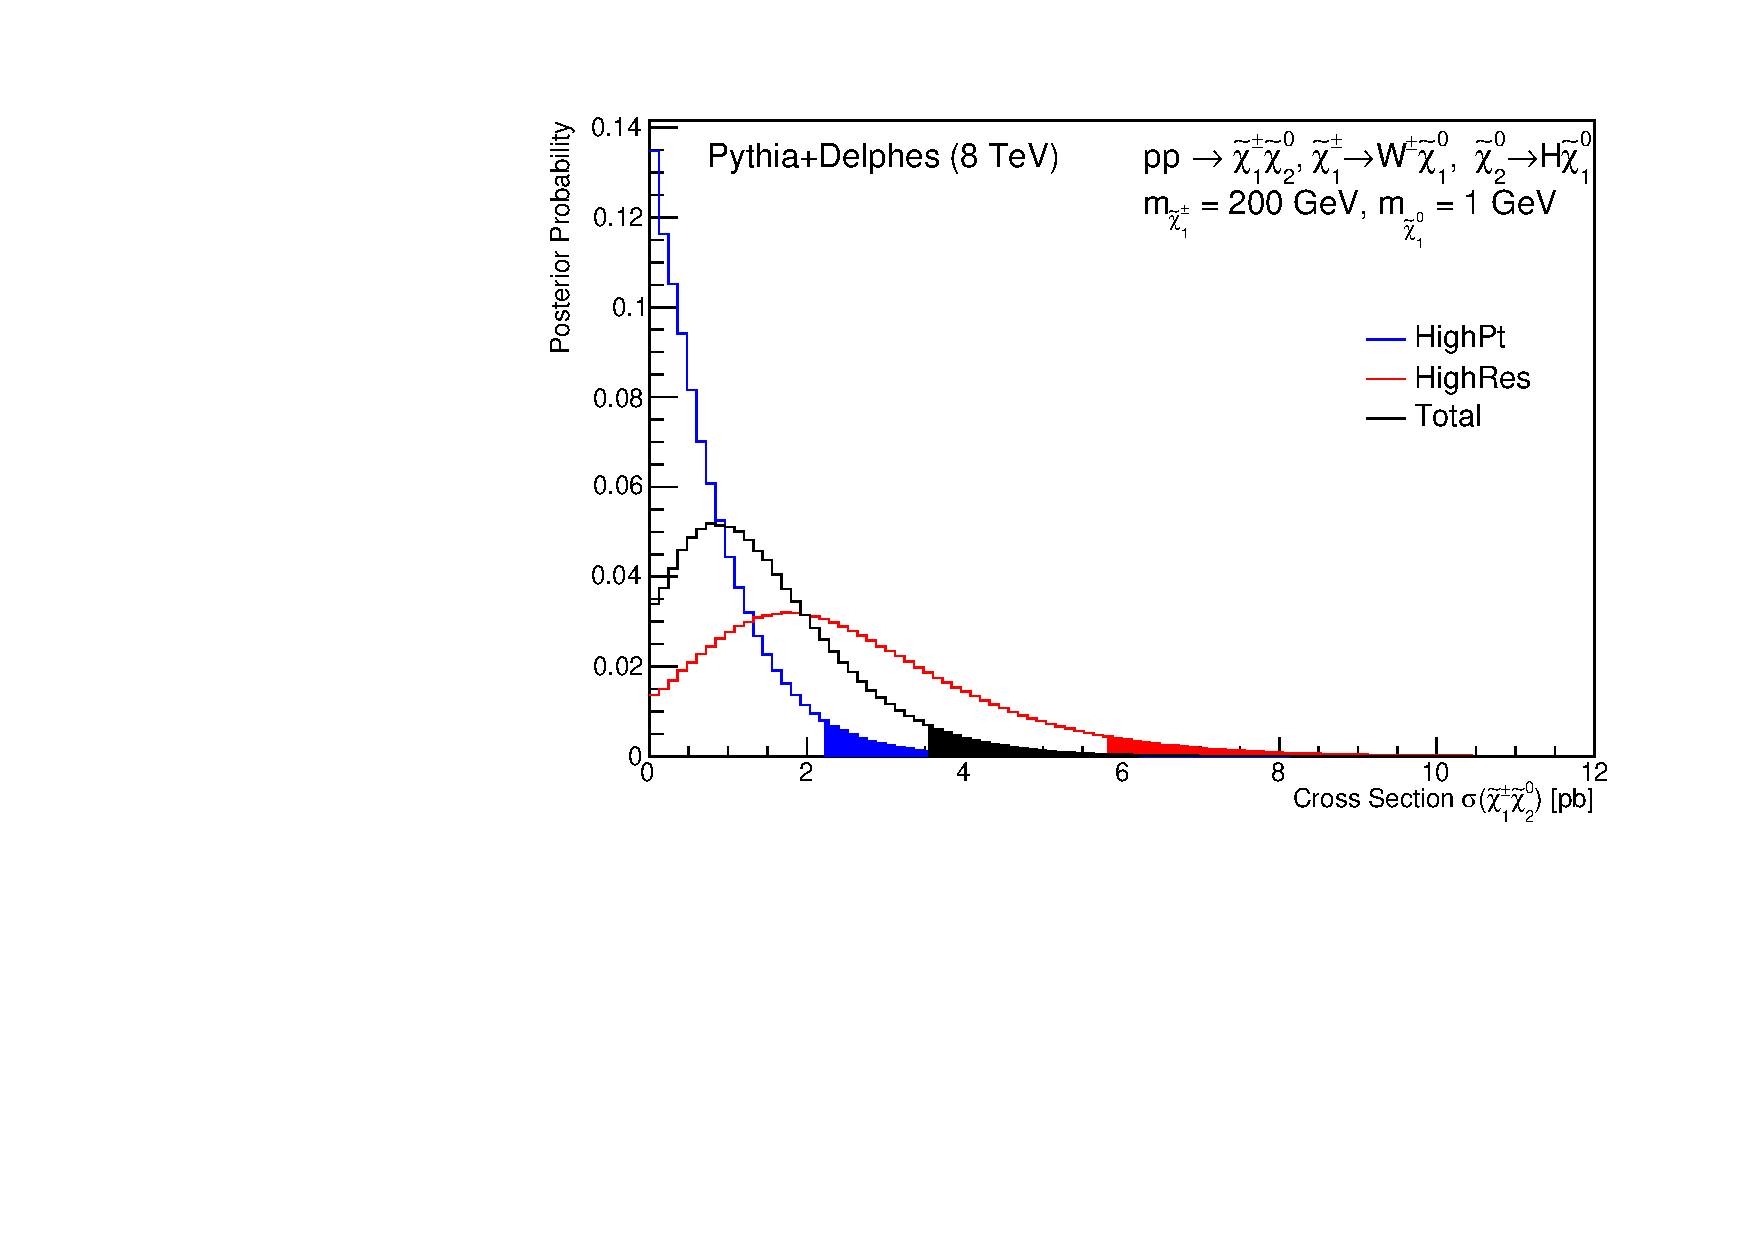
\includegraphics[width=0.45\textwidth]{figs/pheno/posterior_TChiwh_200_1.pdf}
%\caption{\label{fig:TChiwhPosterior200} Posterior probability
 % density functions for the production cross section for the \texttt{HighPt}
 % box (blue), \texttt{HighRes} box (red), and the combination (black). The solid colored region
 % under each curve illustrates the 5\% tail probability. Note, the chosen masses are $m_{\tilde\chi_1^0}=1$\GeV and
 % $m_{\tilde{\chi}_1^{\pm}}=m_{\tilde{\chi}_2^0}=200$\GeV.}
%\end{figure}

\begin{figure}[htb]\centering
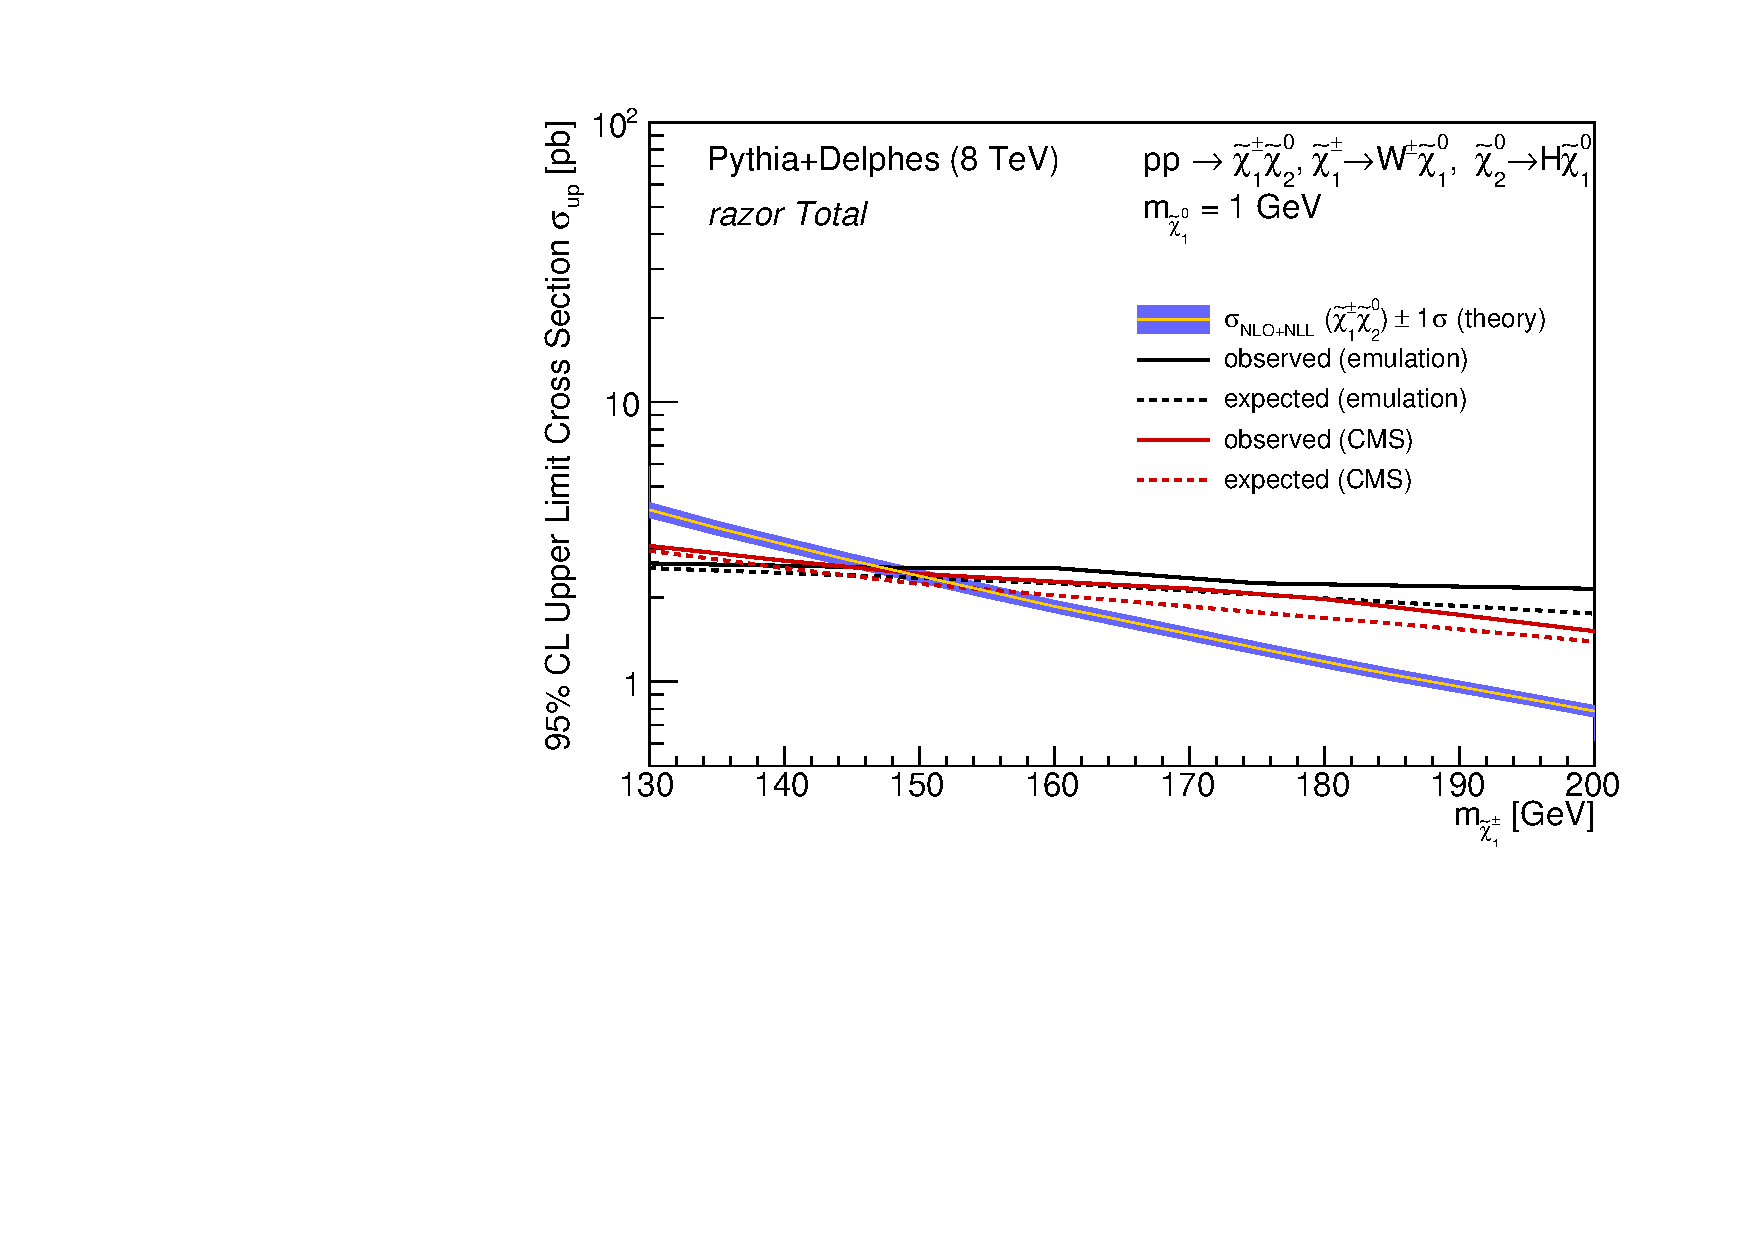
\includegraphics[width=0.45\textwidth]{plots/xsecUL_TChiwh_1_Total.pdf}
\caption{\label{fig:TChiwh1dLimit} Comparison between the CMS
 result (red) and our emulation (black). Note, this scan assumes
 $m_{\chiz_1}=1$\GeV and $m_{\chipm_1}=m_{\chiz_2}$.}
\end{figure}
